
\documentclass[border=10pt]{standalone}
\usepackage{pgfplots}
\pgfplotsset{compat=1.18}
\usepgfplotslibrary{groupplots}
\begin{document}
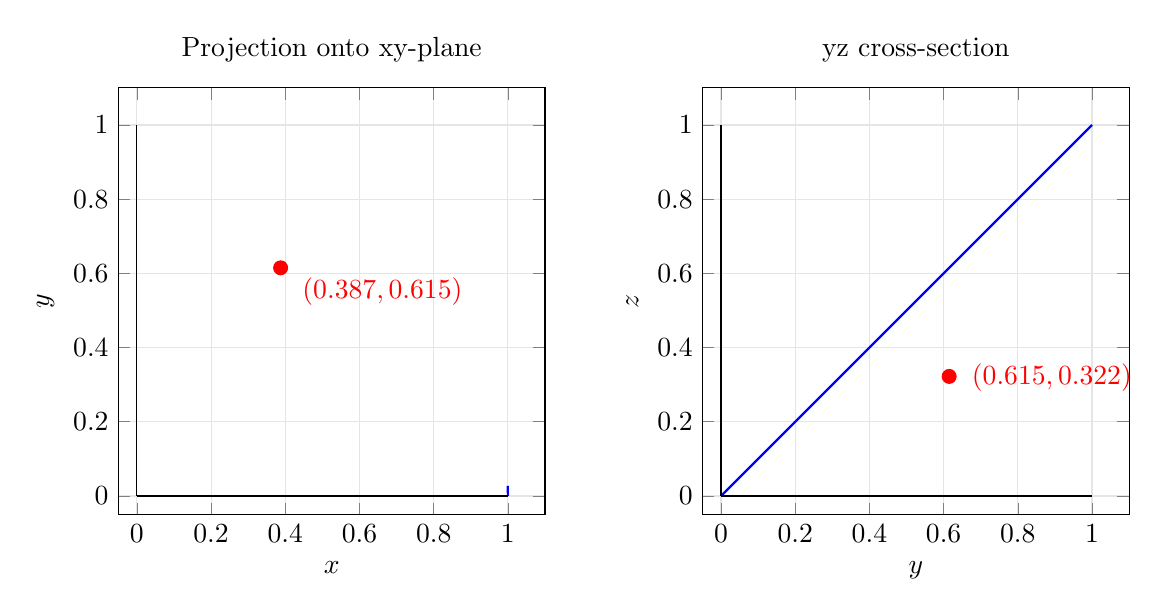
\begin{tikzpicture}
\begin{groupplot}[
    group style={group size=2 by 1, horizontal sep=2cm},
    width=7cm, height=7cm,
    xmin=-0.05, xmax=1.1, ymin=-0.05, ymax=1.1,
    axis equal image,
    grid=major, grid style={gray!20},
]
% Left: xy projection
\nextgroupplot[title={Projection onto xy-plane}, xlabel={$x$}, ylabel={$y$}]
\addplot[domain=0:1.5708, samples=50, fill=cyan!30, draw=cyan!50] 
    ({cos(x)}, {sin(x)}) -- cycle;
\addplot[domain=0:1.5708, samples=50, blue, thick] ({cos(x)}, {sin(x)});
\addplot[domain=0:1, black] ({x}, 0);
\addplot[domain=0:1, black] (0, {x});
\addplot[only marks, mark=*, mark size=2.5pt, red] coordinates {(0.3874, 0.6150)};
\node[red, anchor=west] at (axis cs:0.42, 0.55) {$(0.387, 0.615)$};

% Right: yz view
\nextgroupplot[title={yz cross-section}, xlabel={$y$}, ylabel={$z$}]
\addplot[domain=0:1, samples=50, fill=cyan!30, draw=cyan!50] 
    ({x}, {x}) -- cycle;
\addplot[domain=0:1, samples=50, blue, thick] ({x}, {x});
\addplot[domain=0:1, black] ({x}, 0);
\addplot[domain=0:1, black] (0, {x});
\addplot[only marks, mark=*, mark size=2.5pt, red] coordinates {(0.6150, 0.3223)};
\node[red, anchor=west] at (axis cs:0.65, 0.32) {$(0.615, 0.322)$};
\end{groupplot}
\end{tikzpicture}
\end{document}
